%! TeX program = lualatex
\documentclass[../main.tex]{subfiles}
\begin{document} \section{Beyond \texorpdfstring{\(2\)-by-\(2\)}{2-by-2} matricies}

The general theory for vectors and matricies is called linear algebra. In this section, we formalize our knowledge for \(2\)-by-\(2\) matricies because you will likely encounter similar concepts in high dimensions in courses that work with lots of data. 

We can distill a general concept from solving \(A \vec{x} = \vec{b}\) called the \emph{invertibility of matricies} that \hlmain{transfers our intuition} from real numbers onto matricies.

\faStar{} A square matrix \(A\) is called \hlmain{invertible} if we can find a matrix \(B\) so that \(AB = I\) and \(BA = I\), such a matrix \(B\) is often denoted as \(A^{-1}\). 

\hlsupp{What is invertibility good for?}  Let's say we want to solve \(A \vec{x} = \vec{b}\), and \(A\) happens to be invertible. 
\blanklines{5}

\hlsupp{What is a quick way to determine if \(A\) is invertible?} That's the job for a determinant. The \hlmain{determinant}\footnote{For those who are interested, a general method for calculating determinants is called co-factor expansion.} for a \(2\)-by-\(2\) matrix is \(\det \begin{bmatrix} a & b \\ c & d \end{bmatrix} = ad - bc\).  The determinant for a \(3\)-by-\(3\) matrix is \(\det \begin{bmatrix} a & b & c \\ d & e & f \\ g & h & i\end{bmatrix} = a (ei - fh) - b (di - fg) + c (dh - eg) = aei - afh - bdi + bfg + cdh - ceg \). 
\blanklines{8}

\faStar{} If \(A\) is a square matrix and \(\det(A) \ne 0\), then \(A\) is invertible. 

\begin{example}
  Is \(A = \begin{bmatrix} 0 & -1 & 1 \\ 1 & 9 & -1 \\ 1 & 0 & -1\end{bmatrix}\) invertible?
  \blanklines{10}
\end{example}
\clearpage


\faStar{} We solved a few equations of the form \(\alpha \vec{u} + \beta \vec{v} = \vec{x}(0)\). The general terminology for this operation is called ``write \(\vec{x}(0)\) as a \hlmain{linear combination} of \(\vec{u}\) and \(\vec{v}\).''

\begin{example}
  Write \(\begin{bmatrix} 1 \\ -1 \end{bmatrix}\) as a linear combination of \(\vec{u} = \begin{bmatrix} -1 \\ 0 \end{bmatrix}\) and \(\vec{u} = \begin{bmatrix} 1 \\ 1 \end{bmatrix}\). 

  \blanklines{10}
\end{example}

\faStar{} The following is a summary of matrix operations that we talked about.

\begin{itemize}
  \item The \hlmain{characteristic polynomial} of a square matrix \(A\) is \hlmain{\(\det(A - \lambda I)\)} where \(\lambda\) is an unknown scalar (constant).  The roots of the characteristic polynomial are the eigenvalues for \(A\).  In other words, all \(\lambda\) satisfying \(\det(A - \lambda I) = 0\) is an eigenvalue of \(A\).

  \item We can multiply a matrix \(A\) by a vector \(\vec{v}\). The result of the multiplication \(\vec{u} = A\vec{v}\) is defined by \[u_{i} = \sum_{j=1}^{n} A_{ij}v_{j}.\]  In particular, formulas for matrix-vector multiplication for \(2\)-by-\(2\) and \(3\)-by-\(3\) matricies are
\[
  \begin{bmatrix}
    a & b \\
    c & d 
  \end{bmatrix}
  \begin{bmatrix}
    v_{1} \\ v_{2}
  \end{bmatrix}
  = 
  \begin{bmatrix}
    a v_{1} + b v_{2} \\
    c v_{1} + d v_{2}
  \end{bmatrix}
  \quad\text{and}\quad
  \begin{bmatrix}
    a & b & c \\
    d & e & f \\
    g & h & i
  \end{bmatrix}
  \begin{bmatrix}
    v_{1} \\ v_{2} \\ v_{3}
  \end{bmatrix}
  = 
  \begin{bmatrix}
    a v_{1} + b v_{2} + c v_{3} \\
    d v_{1} + e v_{2} + f v_{3} \\
    g v_{1} + h v_{2} + i v_{3}
  \end{bmatrix}.
\]

  \item We can add matricies of the same size. The result of the addition \(C = A + B\) is defined by \[C_{ij} = A_{ij} + B_{ij}.\]  In particular, the sum of two \(2\)-by-\(2\) matricies is
\[
  \begin{bmatrix}
    a & b \\
    c & d
  \end{bmatrix}
  +
  \begin{bmatrix}
    e & f \\
    g & h
  \end{bmatrix}
  =
  \begin{bmatrix}
    a + e & b + f \\
    c + g & d + h
  \end{bmatrix}.
\]

  \item We can multiply matrices \(A\) and \(B\) if the number of columns in \(A\) is equal to the number of rows in \(B\). Call this common number \(n\). The result of the multiplication \(C = AB\) is defined by 
\[
  C_{ij} = \sum_{k=1}^{n} A_{ik} B_{kj}.
\]
In general, order matters in matrix multiplications, i.e., \(AB \ne BA\).  In particular, the explicit formula for multiplying \(2\)-by-\(2\) matricies is
\[
  \begin{bmatrix}
    a & b \\
    c & d
  \end{bmatrix}
  \begin{bmatrix}
    e & f \\
    g & h
  \end{bmatrix}
  =
  \begin{bmatrix}
    ae + bg & af + bh \\
    ce + dg & cf + dh
  \end{bmatrix}.
\]
\end{itemize}
\clearpage

\section{Vector fields with complex eigenvalues}

We are about to leave discrete models \(\vec{x}(t+1) = A \vec{x}\) and enter the world of systems of differential equations.  Now is a good time to clear up a potential confusion related to vector fields. We compare the \hlmain{purpose} of the matrix \(A\) in 
\[
  \parbox[c]{2in}{\centering sketch the vector field for \(F(\vec{x}) = A \vec{x}\)} \quad\text{versus}\quad \parbox[c]{2in}{\centering sketch the vector field for \(\vec{x}(t+1) = A \vec{x}(t)\)}.
\]
\medskip

\faExclamationTriangle{} In short, the \(A\)'s above \hlwarn{serve different purposes and are NOT interchangeable}. 

Recall that arrows in a vector field visualize changes in a system. 

More formally, the visualization of a linear vector-valued function \(F(x) = A \vec{x}\) is called a linear vector field.  We interpret \(A\) as a ``change matrix'' and think of \(A \vec{x}\) as a change vector.  To draw the vector field, we draw the vector \(A \vec{x}\) \emph{starting at} \(x\) for however many \(\vec{x}\) we want.

However, the \(A\) in a recurrence \(\vec{x}(t+1) = A \vec{x}(t)\) is NOT a ``change matrix.'' The vector \(A \vec{x}(t)\) is the \emph{result} of change, not a change vector. To draw the vector field for the recurrence, we sketch an arrow \emph{from \(\vec{x}\) to \(\vec{x}(t+1)\)} for however many \(\vec{x}\) we want. The change vector is \((A - I) \vec{x}\).

\bigskip

\begin{example}
  Let \(A = \begin{bmatrix} 0 & -1 \\ 1 & 0 \end{bmatrix}\).  Use the provided calculations to sketch the vector field for \(F(\vec{x}) = A \vec{x}\) and \(\vec{x}(t+1) = A \vec{x}(t)\).
  \[
    A \begin{bmatrix}  1 \\ 0 \end{bmatrix} = \begin{bmatrix}    0 \\   1 \end{bmatrix},  \quad
    A \begin{bmatrix}  1 \\ 1 \end{bmatrix} = \begin{bmatrix}   -1 \\   1 \end{bmatrix},  \quad
    A \begin{bmatrix}  0 \\ 1 \end{bmatrix} = \begin{bmatrix}   -1 \\   0 \end{bmatrix},  \quad
    A \begin{bmatrix} -1 \\ 1 \end{bmatrix} = \begin{bmatrix}   -1 \\  -1 \end{bmatrix}.
  \]

  
\begin{center}
  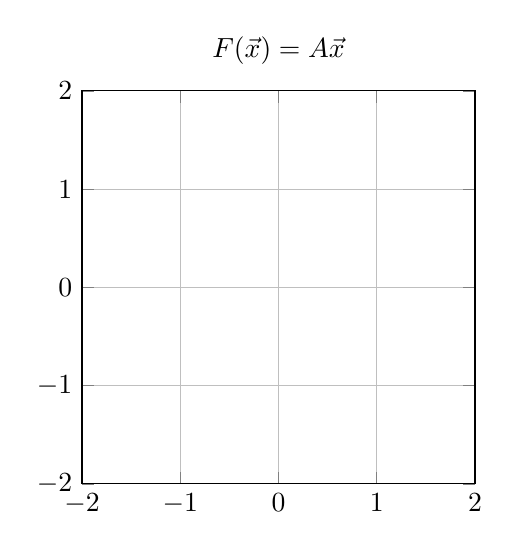
\begin{tikzpicture}
    \begin{axis}[width=3in, xmin=-2, xmax=2, ymin=-2, ymax=2, grid=major, axis equal image, title={\(F(\vec{x}) = A \vec{x}\)}]
    \end{axis}
  \end{tikzpicture}
  \quad
  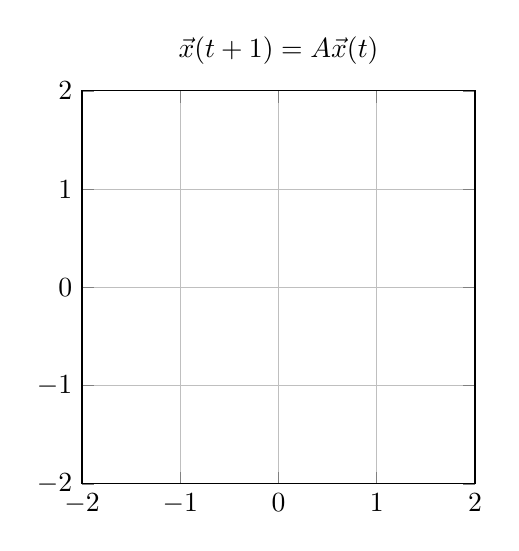
\begin{tikzpicture}
    \begin{axis}[width=3in, xmin=-2, xmax=2, ymin=-2, ymax=2, grid=major, axis equal image, title={\(\vec{x}(t+1) = A \vec{x}(t)\)}]
    \end{axis}
  \end{tikzpicture}
\end{center}
\end{example}

\clearpage

The distinction on the previous page is important because complex eigenvalues for \(F(\vec{x}) = A \vec{x}\) gives us a rough sense of its vector field without any plotting. 

\faStar{} If \(a \pm b i\) are eigenvalues for \(A\) with \(b \ne 0\) (so they are really complex numbers), then

\begin{itemize}
  \item \(a > 0\) implies the vector field spiral \hlmain{away} from the origin, and
  \item \(a < 0\) implies the vector field spiral \hlmain{towards} the origin.
\end{itemize}

\begin{center}
  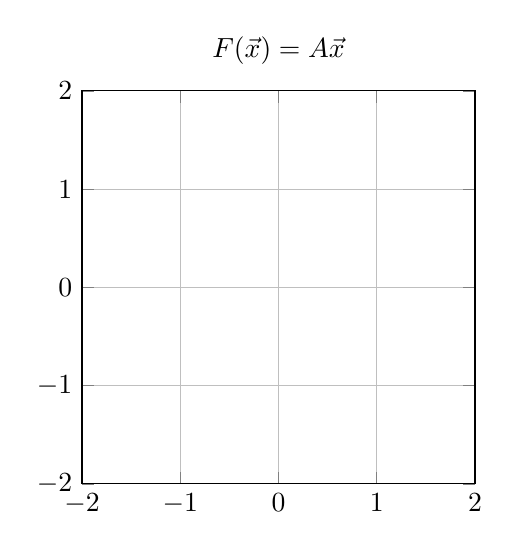
\begin{tikzpicture}
    \begin{axis}[width=3in, xmin=-2, xmax=2, ymin=-2, ymax=2, grid=major, axis equal image, title={\(F(\vec{x}) = A \vec{x}\)}]
    \end{axis}
  \end{tikzpicture}
  \quad
  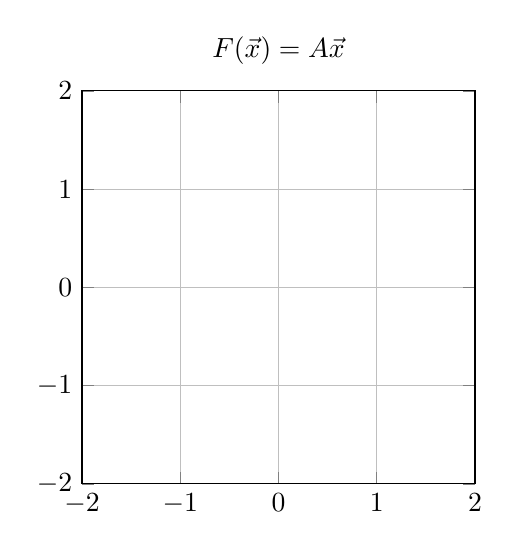
\begin{tikzpicture}
    \begin{axis}[width=3in, xmin=-2, xmax=2, ymin=-2, ymax=2, grid=major, axis equal image, title={\(F(\vec{x}) = A \vec{x}\)}]
    \end{axis}
  \end{tikzpicture}
\end{center}


\end{document}
